\documentclass[10pt,a4paper]{article}
\usepackage[utf8]{inputenc}

% \usepackage{ngerman}  % german documents
\usepackage{graphicx}  % import graphics einbinden
\usepackage{listings}  % support source code listing
\usepackage{amsmath}  % math stuff
\usepackage{amssymb} % 
\usepackage{a4wide} % wide pages
\usepackage{fancyhdr} % nice headers
\usepackage{float}
\usepackage{longtable}
\usepackage{xcolor}
\usepackage{booktabs}
\definecolor{darkpastelgreen}{rgb}{0.01, 0.75, 0.24}
\definecolor{spirodiscoball}{rgb}{0.06, 0.75, 0.99}
\definecolor{smalt}{rgb}{0.0, 0.2, 0.6}
\definecolor{armygreen}{rgb}{0.29, 0.33, 0.13}
\definecolor{awesome}{rgb}{1.0, 0.13, 0.32}
\definecolor{bittersweet}{rgb}{1.0, 0.44, 0.37}
\definecolor{bananayellow}{rgb}{1.0, 0.88, 0.21}
\definecolor{blue}{rgb}{0.0, 0.0, 1.0}
\definecolor{red}{rgb}{1.0, 0.0, 0.0}
\definecolor{green}{rgb}{0.0, 1.0, 0.0}

% for multiple figures
\usepackage{subcaption}


\lstset{basicstyle=\footnotesize,language=Python,breaklines=true,numbers=left, numberstyle=\tiny, stepnumber=5,firstnumber=0, numbersep=5pt} % set up listings
\pagestyle{fancy}             % header
\setlength{\parindent}{0pt}   % no indentation
 

\usepackage[pdfpagemode=None, colorlinks=true,  % url coloring
           linkcolor=blue, urlcolor=blue, citecolor=blue, plainpages=false, 
           pdfpagelabels,unicode]{hyperref}
           
% change enums style: first level (a), (b), (c)           
\renewcommand{\labelenumi}{(\alph{enumi})}
\renewcommand{\labelenumii}{(\arabic{enumii})}

\newcommand{\norm}[1]{\left\lVert#1\right\rVert}

%lecture name
\newcommand{\lecture}{
	Bioinformatics III
}           

%assignment iteration
\newcommand{\assignment}{
	Ninth Assignment
}


%set up names, matricle number, and email
\newcommand{\authors}{
  \begin{tabular}{rl}
    \href{mailto:s8tbscho@stud.uni-saarland.de}{Thibault Schowing} & (2571837)\\
    \href{mailto:wiebkeschmitt@outlook.de}{Wiebke Schmitt} & (2543675)
  \end{tabular}
}

% use to start a new exercise
\newcommand{\exercise}[1]
{
  \stepcounter{subsection}
  \subsection*{Exercise \thesubsection: #1}

}

\begin{document}
\title{\Large \lecture \\ \textbf{\normalsize \assignment}}
\author{\authors}

\setlength \headheight{25pt}
\fancyhead[R]{\begin{tabular}{r}\lecture \\ \assignment \end{tabular}}
\fancyhead[L]{\authors}


\setcounter{section}{9} % modify for later sheets, i.e. 2, 3, ...
%\section{Introduction to Python and some Network Properties} % optional, note that section invocation sets the section counter + 1, so adapt the setcounter command
\maketitle

%EXERCICE 1
\exercise{Extreme Pathways and Steady State Flux Distribution. Paper-based}

\begin{enumerate}

% A
\item \textbf{Construct the stoichiometric matrix:}\\ 

%\lstinputlisting[label=qtew-1, caption={Data Matrix class script}] {../Scripts/data\string_matrix.py}


\begin{figure}[H]
	\centering
	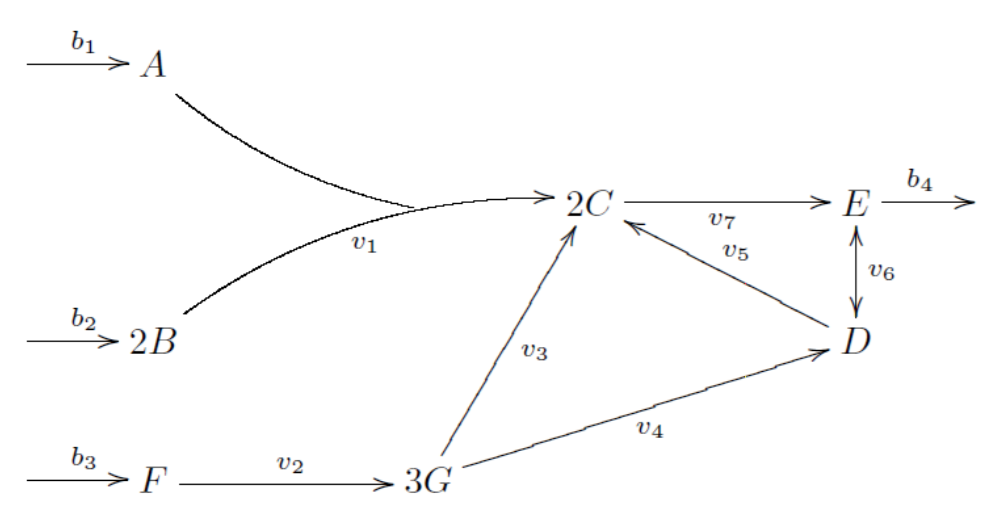
\includegraphics[width=0.7\linewidth]{img/ex1}
	\caption{Reaction network to derive extreme pathways from.}
	\label{fig:ex1}
\end{figure}


\begin{table}[H]
	\centering
	\caption{Stochiometric Matrix}
	\label{stociometric1}
	\begin{tabular}{|l|l|l|l|l|l|l|l|l|l|l|l|l|}
		\hline
		& v1 & v2 & v3 & v4 & v5 & v6 & v6 & v7 & b1 & b2 & b3 & b4 \\ \hline
		A & -1 & 0  & 0  & 0  & 0  & 0  & 0  & 0  & 1  & 0  & 0  & 0  \\ \hline
		B & -2 & 0  & 0  & 0  & 0  & 0  & 0  & 0  & 0  & 1  & 0  & 0  \\ \hline
		C & 2  & 0  & 2  & 0  & 2  & 0  & 0  & -2 & 0  & 0  & 0  & 0  \\ \hline
		D & 0  & 0  & 0  & 1  & -1 & 1  & -1 & 0  & 0  & 0  & 0  & 0  \\ \hline
		E & 0  & 0  & 0  & 0  & 0  & -1 & 1  & 1  & 0  & 0  & 0  & -1 \\ \hline
		F & 0  & -1 & 0  & 0  & 0  & 0  & 0  & 0  & 0  & 0  & 1  & 0  \\ \hline
		G & 0  & 3  & -3 & -3 & 0  & 0  & 0  & 0  & 0  & 0  & 0  & 0  \\ \hline
	\end{tabular}
\end{table}



%B
\item \textbf{Calculate from the stoichiometric matrix the extreme pathways. Give pathways as formulas.} \\

\item \textbf{Formulate the pathway length matrix. Which information does it provide (diagonal vs off-diagonal entries?}\\

\item \textbf{Formulate the reaction particiaption matrix. Which information does it provide?}\\

\item \textbf{Cut-set.} \textit{A reaction or a set of reactions are essential for the network, when there is no output if this reactions are blocked. List all those reactions.}\\

\item \textbf{Biomass producation.}\textit{Now assume that the potential input into the network through b1, b2, and b3, i.e., the sum of the fluxes through these reactions is limited to 5 units. How must this input be distributed onto these reactions to give the highest output through b4?}\\





\end{enumerate}


%\newpage
%\lstinputlisting[label=qtew-1, caption={boolean\textunderscore network.py}] {../Scripts/boolean\string_network.py}
%\newpage
%\lstinputlisting[label=qtew-1, caption={Main function that tests the boolean network}] {../Scripts/main\string_boolean.py}




% NEW EXERCICE
\newpage
\exercise{Hands-on with COnstraint-Based Reconstruction and Analysis (COBRA) in Python.}

\begin{enumerate}
	
	\item \textbf{Provide formulas of the reactions participating in the chain.}
	
	\lstinputlisting[language={}]{../Scripts/Output.txt}
	
	
	
	\item \textbf{Fill in the stoichiometry matrix.}
	
	\begin{table}[H]
		\centering
		\caption{Stochiometry matrix}
		\label{my-label}
		\begin{tabular}{|l|l|l|l|l|l|l|l|l|l|l|}
			\hline
			& HEX1 & PGI & PFK & FBA & TPI & GAPD & PGK & PGM & ENO & PYK \\ \hline
			ATP   & -1   &     & -1  &     &     &      & -1  &     &     & 1   \\ \hline
			GLC   & -1   &     &     &     &     &      &     &     &     &     \\ \hline
			ADP   & 1    &     & 1   &     &     &      & 1   &     &     & -1  \\ \hline
			G6P   & 1    & -1  &     &     &     &      &     &     &     &     \\ \hline
			H     & 1    &     & 1   &     &     & 1    &     &     &     & -1  \\ \hline
			F6P   &      & 1   & -1  &     &     &      &     &     &     &     \\ \hline
			FDP   &      &     & 1   & -1  &     &      &     &     &     &     \\ \hline
			DHAP  &      &     &     & 1   & -1  &      &     &     &     &     \\ \hline
			G3P   &      &     &     & 1   & 1   & -1   &     &     &     &     \\ \hline
			NAD   &      &     &     &     &     & -1   &     &     &     &     \\ \hline
			PI    &      &     &     &     &     & -1   &     &     &     &     \\ \hline
			13DPG &      &     &     &     &     & 1    & 1   &     &     &     \\ \hline
			NADH  &      &     &     &     &     & 1    &     &     &     &     \\ \hline
			3PG   &      &     &     &     &     &      & -1  & 1   &     &     \\ \hline
			2PG   &      &     &     &     &     &      &     & -1  & -1  &     \\ \hline
			PEP   &      &     &     &     &     &      &     &     & 1   & -1  \\ \hline
			H2O   &      &     &     &     &     &      &     &     & 1   &     \\ \hline
			PYR   &      &     &     &     &     &      &     &     &     & 1   \\ \hline
		\end{tabular}
	\end{table}
	
	
	
	\item \textbf{Create the model for the given chain of reactions. Provide the number of reactions, metabolites and genes in it. (Python) }\\
	
	We obtain 10 reactions implying 16 genes and 18 metabolites. Code below.
	
	
	
	\lstinputlisting[label=lsdddt-1, caption={Correlation network}] {../Scripts/Assignment9.py}
	
	
\end{enumerate}



% NEW EXERCICE
\newpage
\exercise{asdf}
\begin{enumerate}
	
	% A
	\item \textbf{asdf}\\
	
	%\lstinputlisting[label=lsdddt-1, caption={Correlation network}] {../Scripts/network.py}
	
	
	% B
	\item \textbf{asdf}

\end{enumerate}


\end{document}